\section{Section A}
\subsection{(i)}
Laplace transform is a technique used to solve differential equations [1].
\begin{align*}
    \boxed{\laplace{x(t)} = X(s) = \int_{0}^{\infty}x(t)e^{-st}dt}
\end{align*}
The idea is to take the laplace transform on both sides of the differential equation to convert everything from $x(t)$ into $X(s)$. Then, move $X(s)$ into one side of the equation and perform an inverse laplace transform to obtain $x(t)$ again.

\subsection{(ii)}
Laplace transform is useful in Signal and Systems because all of the LTI systems can be modelled in differential equation form. And since Laplace transform is the easiest tool to analyze a differential equation, we can analyze the behavior of an LTI system easily by first converting it into a differential equation and then taking the Laplace transform.

Another key point is that most LTI systems are expressed in convolution form as well, $y(t) = x(t) * h(t)$. It will take a lot of time to solve the convolution sum manually, hence Laplace transform is also used here to ease our workload, because when being transformed into the s-domain, convolution will become multiplication.
\begin{align*}
    \boxed{y(t)=x(t) * h(t) \Leftrightarrow Y(s)=X(s)H(s)}
\end{align*}

\subsection{(iii)}
The difference between time-domain and s-domain is that in time-domain, $x(t)$ is in the form of differential equation, but in s-domain, $X(s)$ is in the form of algebraic equation.
\begin{align*}
    \boxed{\laplace{x'(t)}=sX(s)-x(0)}\\
    \boxed{\laplace{x''(t)}=s^2X(s)-sx(0)-x'(0)}
\end{align*}
Since it is easier to analyze algebraic equation than differential equation, the s-domain is preferable for analysis.

\subsection{(iv)}
In RLC transient analysis, the voltage source/current source is often times a unique function. Since it's not 0, we cannot use the standard method of assuming $x(t)=e^{st}$. Hence, Laplace transform is a necessary technique to be learned to solve complex RLC equations.

Furthermore, a table of Laplace transform equations has been widely developed [2]. This makes using Laplace transform to solve RLC equations extremely convenient.

\subsection{(v)}
A pole, $s=p$ is a value of $s$ in which $X(s)$ blows up to infinity. Generally, the Laplace transform of our function $X(s)$ will be in the form of $\frac{A(s)}{B(s)}$, and the pole is generally the value which makes the denominator 0 ($B(p)=0$).

\begin{align*}
    \boxed{\lim_{s \rightarrow p}X(s) = \infty}
\end{align*}

A circuit is considered stable if its response die out, or in other words, $x(t)$ goes to 0. We can use the pole to determine whether if the circuit will die out or not. The rule of thumb is that \textbf{if the pole contains negative real parts, then the circuit will be stable. If the pole contains positive real parts, then the circuit will be unstable [1].}

To uncover why this rule of thumb works, We need to understand another concept of Laplace transform, which is that Laplace transform is not just used to solve differential equations, but it is also used to \textbf{convert any function into a series of exponential sums}.
\begin{align*}
    \boxed{x(t) = C_1e^{s_1t} + C_2e^{s_2t} + C_3e^{s_3t} + \cdots}
\end{align*}
Where $s_1, s_2, s_3, \cdots$ are the poles we obtain from taking the laplace transform (see Appendix for the mathematical proof). If one of the poles contains a positive real part, say $e^{20t}$, then as t increases to infinity, the entire term will blow up to infinity. Similarly, if all of the poles consist of negative real parts, say $e^{-20t}$, then as t increase to infinity, the whole function will decrease to 0.

The final caveat left is the proof of why $s_1, s_2, s_3, \cdots$ are poles of the laplace transform. The proof of this is attached in the Appendix.

\section{Section B}
\subsection{(i)}

\begin{figure}[H]
    \centering
    \begin{circuitikz}[american, scale=1.2, transform shape]
        % Main loop components
        \draw (0,0) to[V, l={$v_s(t) = 100u(t)$}, invert] (0,3)
              to[R, l={$R = 20\,\Omega$}] (2.5,3)
              to[L, l={$L = 0.5\text{ H}$}] (5,3)
              to[C, l={$C = 200\,\mu\text{F}$}] (5,0)
              -- (0,0);
        
        % Voltage polarity labels for Capacitor (drawn manually for absolute version-compatibility)
        \node[anchor=east, primarynavy, font=\small] at (4.6, 2.3) {$+$};
        \node[anchor=east, primarynavy, font=\small] at (4.6, 1.5) {$v_c(t)$};
        \node[anchor=east, primarynavy, font=\small] at (4.6, 0.7) {$-$};
        
        % Clockwise loop current arrow
        \draw[thin, -{Stealth[scale=0.8]}, accentteal] (2.5,1.5) ++(150:0.5) arc (150:-150:0.5) node[midway, above=1pt, font=\small] {$i(t)$};
        
        % Styled initial conditions annotation card
        \node[draw=lightgrey, fill=softbg, rounded corners=3pt, thick, anchor=north, align=left, font=\small\sffamily\color{slategrey}, inner sep=6pt] at (2.5,-0.4) {
            \textbf{\color{primarynavy}Initial Conditions:} \\
            $i(0^-) = 0\text{ A}$ \\
            $v_c(0^-) = 0\text{ V}$
        };
    \end{circuitikz}
    \vspace{0.8cm}
    \label{fig:rlc_circuit}
\end{figure}

\begin{align*}
    v_l(t) &= i'(t)L \\
    i(t) &= v_c'(t)C\\
    v_c'(t) &= \frac{1}{C}i(t)\\
    v_c(t) &= \int_{0}^{t} \frac{1}{C} i(t)\\ \\
    v_s(t) &= i(t)R + v_l(t) + v_c(t)\\
    &= i(t)R + i'(t)L + \int_{0}^{t} \frac{1}{C} i(t)\\ \\
    v_s'(t) &= i'(t)R + i''(t)L + \frac{1}{C}i(t)\\
    100\impulse{t} &= 20i' + \frac{1}{2}i'' + \frac{1}{200\mu}i\\
    &\boxed{100\impulse{t} = \frac{1}{2}i'' + 20i' + \frac{1}{200\mu}i}
\end{align*}

\subsection{(ii)}

\begin{tcolorbox}[colback=softbg, colframe=accentteal, title={}, arc=3pt, outer arc=3pt, boxrule=0.8pt, leftrule=4pt, fonttitle=\bfseries\sffamily]
\begin{align*}
    v_s(0^-) &= v_R(0^-) + v_L(0^-) + v_c(0^-) \\
    v_s(0^-) &= i(0^-)R + L \cdot i'(0^-) + v_c(0^-) \\
    0 &= (0)(20) + 0.5 \cdot i'(0^-) + 0 \\
    0 &= 0.5 \cdot i'(0^-) \\
    \implies i'(0^-) &= 0
\end{align*}
\end{tcolorbox}
\begin{align*}
    100\impulse{t} &= \frac{1}{2}i'' + 20i' + \frac{1}{200\mu}i\\
    100 &= \frac{1}{2}\left(s^2I(s)-si(0^-)-i'(0^-)\right) + 20\left(sI(s)-i(0^-)\right) + \frac{1}{200\mu}I(s) \\
    &= \frac{1}{2}\left(s^2I(s) - s(0) - 0\right) + 20\left(sI(s) - 0\right) + \frac{1}{200\mu}I(s) \\
    &= \frac{1}{2}s^2I(s) + 20sI(s) + \frac{1}{200\mu}I(s) \\
    &\boxed{20000\mu = 100\mu s^2 I(s) + 4000\mu s I(s) + I(s)}
\end{align*}

\subsection{(iii)}
\begin{align*}
    20000\mu &= 100\mu s^2 I(s) + 4000\mu s I(s) + I(s)\\
    I(s) &= \frac{0.02}{0.0001 s^2 + 0.004s + 1}\\
    & \boxed{I(s) = \frac{200}{s^2 + 40s + 10000}}
\end{align*}

\subsection{(iv)}
Since the denominator cannot be factorized ($40^2 - 4(10000) \leq 0$), we have to complete the square to convert the fraction into a form that can be processed by the inverse laplace transform.
\begin{align*}
    \frac{200}{s^2 + 40s + 10000} &= \frac{200}{s^2 + 40s + 400 - 400 + 10000}\\
    &= \frac{200}{(s+20)^2 + 9600}\\
    &= \frac{5}{\sqrt{6}} \frac{40\sqrt{6}}{(s-(-20))^2 + (40\sqrt{6})^2}\\
    &\boxed{I(s)=\frac{5}{\sqrt{6}} \frac{40\sqrt{6}}{(s-(-20))^2 + (40\sqrt{6})^2}}
\end{align*}

\subsection{(v)}
From the laplace transform table, we know that $\laplace{e^{\alpha t}\sin(bt)u(t)}=\frac{b}{(s-\alpha)^2+b^2}$ 
\begin{align*}
    I(s)&=\frac{5}{\sqrt{6}} \frac{40\sqrt{6}}{(s-(-20))^2 + (40\sqrt{6})^2}\\
    &\boxed{i(t) = \frac{5}{\sqrt{6}}e^{-20t}\sin(40\sqrt{6}t)u(t)}
\end{align*}

\subsection{(vi)}
\begin{align*}
    100\impulse{t} &= \frac{1}{2}i'' + 20i' + \frac{1}{200\mu}i\\
    b^2 - 4ac &= 20^2 - 4(1/2)(1/200\mu)\\
    &= -9600 (< 0)\\
    &\boxed{\therefore \text{under-damped}}
\end{align*}

\newpage

\section{Section C}

\begin{figure}[H]
    \centering
    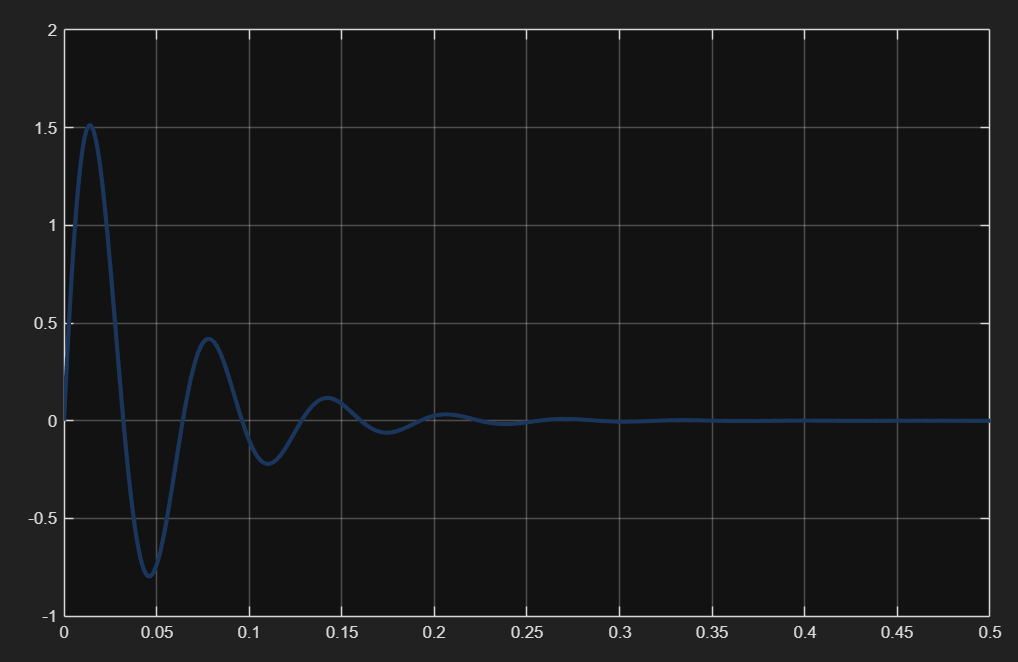
\includegraphics[width=0.85\textwidth]{images/image.png}
    \label{fig:matlab_current_plot}
\end{figure}

\begin{lstlisting}[style=matlabstyle]
t = 0:0.0005:0.5; % time from 0 to 0.5 seconds with 0.5ms increment
i_t = 5 * exp(-20 * t) .* sin(40 * sqrt(6) * t) / sqrt(6); % formula for i(t)
plot(t, i_t, 'Color', [26/255, 54/255, 93/255], 'LineWidth', 2.5, 'DisplayName', 'Transient Current i(t)'); % plot the graph out
grid on; % show grid
\end{lstlisting}

\section{Section D}
Mathematically speaking, the analysis of the RLC circuit is just an analysis of a second order differential equation. Hence, the solution used here can be easily extended into any other engineering applications that involves second order differential equations. The following are two examples of such applications:
\begin{enumerate}
    \item \textbf{Mass Spring Damping System}
    In mechanical engineering, a mass connected to a spring and damper can be modeled as shown in Fig.~\ref{fig:translational_system}, and is described by the following differential equation [3]:
    \begin{figure}[H]
        \centering
        \begin{tikzpicture}[scale=1.0, transform shape]
            % Wall (Hatched)
            \draw[thick] (0,0) -- (0,2);
            \foreach \y in {0, 0.25, 0.5, 0.75, 1.0, 1.25, 1.5, 1.75, 2.0}
                \draw (0,\y) -- (-0.2,\y-0.2);
                
            % Ground line
            \draw[thick] (0,0) -- (5,0);
            \foreach \x in {0.2, 0.6, 1.0, 1.4, 1.8, 2.2, 2.6, 3.0, 3.4, 3.8, 4.2, 4.6}
                \draw (\x,0) -- (\x-0.1,-0.1);
                
            % Mass Block (m)
            \draw[draw=primarynavy, fill=softbg, thick] (2.2, 0.2) rectangle (3.8, 1.8);
            \node[color=primarynavy, font=\sffamily\bfseries] at (3, 1) {$m$};
            
            % Wheels
            \draw[draw=primarynavy, fill=white, thick] (2.6, 0.1) circle (0.1);
            \draw[draw=primarynavy, fill=white, thick] (3.4, 0.1) circle (0.1);
            
            % Spring (zig-zag)
            \draw[thick] (0, 1.3) -- (0.4, 1.3)
                -- (0.6, 1.5) -- (0.8, 1.1) -- (1.0, 1.5) -- (1.2, 1.1) -- (1.4, 1.5) -- (1.6, 1.1) -- (1.8, 1.3)
                -- (2.2, 1.3);
            \node[font=\small\sffamily, color=accentteal, above=2pt] at (1.1, 1.5) {$k$};
            
            % Damper (cylinder & piston)
            \draw[thick] (0, 0.7) -- (0.6, 0.7);
            \draw[thick] (0.6, 0.5) -- (0.6, 0.9) -- (1.6, 0.9);
            \draw[thick] (0.6, 0.5) -- (1.6, 0.5);
            \draw[thick] (1.3, 0.7) -- (2.2, 0.7);
            \draw[thick] (1.3, 0.6) -- (1.3, 0.8);
            \node[font=\small\sffamily, color=accentteal, below=2pt] at (1.1, 0.5) {$c$};
            
            % External Force arrow (F_ext)
            \draw[ultra thick, -{Stealth[scale=1.2]}, primarynavy] (3.8, 1) -- (4.8, 1) node[midway, above, font=\small\sffamily\bfseries] {$F_{ext}$};
            
            % Displacement indicator x(t)
            \draw[thin, -{Stealth[scale=1.0]}, slategrey] (3, 2.1) -- (3.8, 2.1) node[midway, above, font=\small\sffamily] {$x(t)$};
            \draw[dotted, slategrey] (3, 1.8) -- (3, 2.2);
        \end{tikzpicture}
        \caption{Translational Mass-Spring-Damper System schematic.}
        \label{fig:translational_system}
    \end{figure}
    \begin{align*}
        \sum F &= ma\\
        \text{damping force} + \text{restoring force} + \text{external force} &= mx''\\
        -cx' - kx + F_{ext} &= mx''\\
        \boxed{F_{ext} = mx'' + cx' + kx}
    \end{align*}
    We can compare the like terms to realize that we can directly apply the solution techniques used in the RLC circuit into analyzing the mass spring damping system, because \textbf{the equation is of the same form, the only thing that changes are the variable names}.

    \begin{tabular}{|c|c|c|}
        \hline
        RLC & Mass Spring Damping System \\
        \hline
        $v_s'$ & $F_{ext}$ \\
        \hline
        $L$ & $m$ \\
        \hline
        $R$ & $c$ \\
        \hline
        $1/C$ & $k$ \\
        \hline
        $i$ & $x$ \\
        \hline
    \end{tabular}

    \item \textbf{DC Motor Torque}
    
    To design a DC Motor, the DC motor torque will have to be finely analyzed. The motor shaft rotational load can be modeled as shown in Fig.~\ref{fig:rotational_system}, and the torque is expressed by the following formula [3]:
    \begin{figure}[H]
        \centering
        \begin{tikzpicture}[scale=1.0, transform shape]
            % Fixed wall on the left
            \draw[thick] (0, 0.5) -- (0, 2.5);
            \foreach \y in {0.5, 0.75, 1.0, 1.25, 1.5, 1.75, 2.0, 2.25, 2.5}
                \draw (0,\y) -- (-0.2,\y-0.2);
                
            % Rotational shaft
            \draw[thick] (0, 1.5) -- (0.8, 1.5);
            
            % Torsional Spring (k)
            \draw[thick, accentteal] (0.8, 1.5) -- (1.0, 1.8) -- (1.2, 1.2) -- (1.4, 1.8) -- (1.6, 1.2) -- (1.8, 1.5);
            \draw[thick] (1.8, 1.5) -- (2.3, 1.5);
            \node[font=\small\sffamily, color=accentteal, above=3pt] at (1.3, 1.8) {$k$};
            
            % Rotational Damper / Friction (b)
            \draw[thick] (2.3, 1.5) -- (2.6, 1.5);
            \draw[draw=primarynavy, fill=softbg, thick] (2.6, 1.2) rectangle (3.0, 1.8);
            \draw[thick, draw=accentteal, fill=accentteal] (2.8, 1.3) rectangle (2.85, 1.7);
            \draw[thick] (2.85, 1.5) -- (3.4, 1.5);
            \node[font=\small\sffamily, color=accentteal, below=2pt] at (2.8, 1.2) {$b$};
            
            % Inertia Disk (J)
            \draw[draw=primarynavy, fill=softbg, thick] (3.4, 1.5) -- (3.8, 1.5);
            \draw[draw=primarynavy, fill=softbg, thick] (3.8, 1.5) ellipse (0.25 and 0.8);
            \node[color=primarynavy, font=\sffamily\bfseries] at (3.8, 1.5) {$J$};
            
            % Torque arrow T_ext
            \draw[ultra thick, -{Stealth[scale=1.2]}, primarynavy] (3.8, 2.2) arc[start angle=90, end angle=-30, radius=0.6] node[midway, right=1pt, font=\small\sffamily\bfseries] {$T_{ext}$};
            
            % Angular displacement arrow \theta(t)
            \draw[thin, -{Stealth[scale=1.0]}, slategrey] (3.8, -0.2) arc[start angle=-90, end angle=-200, radius=0.5] node[midway, left=1pt, font=\small\sffamily] {$\theta(t)$};
        \end{tikzpicture}
        \caption{Rotational Torsional Spring-Mass-Damper (DC Motor) schematic.}
        \label{fig:rotational_system}
    \end{figure}
    \begin{align*}
        \sum T &= J\alpha \\
        \text{damping torque} + \text{torsional spring torque} + \text{external torque} &= J\theta'' \\
        -b\theta' - k\theta + T_{ext} &= J\theta'' \\
        \boxed{T_{ext} = J\theta'' + b\theta' + k\theta}
    \end{align*}
    Just like the previous application, comparing the like terms reveals that we can directly apply the RLC solution techniques to analyze rotational shaft oscillations, because the mathematical form is identical.

    \begin{tabular}{|c|c|c|}
        \hline
        RLC & Rotational Mechanical System \\
        \hline
        $v_s'$ & $T_{ext}$ \\
        \hline
        $L$ & $J$ \\
        \hline
        $R$ & $b$ \\
        \hline
        $1/C$ & $k$ \\
        \hline
        $i$ & $\theta$ \\
        \hline
    \end{tabular}
\end{enumerate}

\section{Section E}
\begin{enumerate}
    \item \textbf{SDG 11: Sustainable Cities and Communities [4]: } We can utilize Laplace transform to identify the stability of an RLC circuit. With it, we can modify the values of R, L, and C to achieve our desired behavior for the RLC circuit. In most cases, a finely tuned RLC circuit can be used as a low pass filter, which is used to filter out dangerous high frequency input signals to prevent damage to our electronic appliances, thereby making cities and communities sustainable.
    \item \textbf{SDG 9: Industry, Innovation and Infrastructure [5]: } Most industrial electronic devices (microchips) are extremely sensitive to signal surges. By analyzing the RLC circuit using Laplace Transform Techniques and pole analysis, we can predict the transient behavior of the circuit (identify the peak voltage surges) and implement appropriate protective measurements. With the proper protective devices in place, we can ensure a highly resilient and sustainable industrial infrastructure that keeps hospitals, factories, and schools running safely without interruptions.
\end{enumerate}

\newpage
\section{Appendix: Proof of Exponential Coefficients as Poles}
\label{sec:appendix}

In Section A (v), we assumed that all functions can be converted into a sum of exponentials.
\begin{align*}
    x(t) = \sum_{i=1}^{N} C_i e^{s_i t} u(t) = C_1 e^{s_1 t} u(t) + C_2 e^{s_2 t} u(t) + C_3 e^{s_3 t} u(t) + \cdots
\end{align*}
We wish to prove that these coefficients $s_1, s_2, s_3, \dots$ are the poles of the Laplace transform of $x(t)$. We can do so by taking the Laplace transform of the entire equation.

\begin{align*}
    x(t) &= \sum_{i=1}^{N} C_i e^{s_i t} u(t)\\
    X(s) &= \laplace{\sum_{i=1}^{N} C_i e^{s_i t} u(t)}\\
    &= \sum_{i=1}^{N} C_i \laplace{e^{s_i t} u(t)} \\
    &= \sum_{i=1}^{N} \frac{C_i}{s - s_i}
\end{align*}
Recall that poles are the values of $s$ which makes $X(s)$ blow up to infinity. From the equation derived above, we can see that when $s=s_i$, $X(s)$ will blow up.
\begin{align*}
    \text{if } s = s_i:\\
    X(s) &= \sum_{i=1}^{N} \frac{C_i}{s - s_i} \\
    & = \sum_{i=1}^{N} \frac{C_i}{s_i - s_i} \\
    & = \sum_{i=1}^{N} \frac{C_i}{0}\\
    & = \infty
\end{align*}
\textbf{Hence, it is then proven that whenever $s = s_i$, $X(s)$ will blow up, hence $s_i = s_1, s_2, s_3, \cdots$ are the poles of the Laplace transform of $x(t)$.}

\newpage
\section{References}
\begin{enumerate}[label={[\arabic*]}, leftmargin=*, itemsep=6pt]
    \item TutorialsPoint. (n.d.). \textit{Signals and Systems}. Retrieved May 30, 2026, from \url{https://www.tutorialspoint.com/signals_and_systems/laplace_transforms.htm}
    \item Dawkins, P. (n.d.). \textit{Laplace Transform Table}. Paul's Online Notes (Lamar University). Retrieved May 30, 2026, from \url{https://tutorial.math.lamar.edu/Classes/DE/Laplace_Table.aspx}
    \item Swarthmore College Department of Engineering. (n.d.). \textit{Linear Physical Systems Analysis: Analogous Electrical and Mechanical Systems}. Retrieved May 30, 2026, from \url{https://lpsa.swarthmore.edu/Analogs/ElectricalMechanicalAnalogs.html}
    \item United Nations. (2015). \textit{Goal 11: Make cities and human settlements inclusive, safe, resilient and sustainable}. United Nations Sustainable Development Goals. Retrieved May 30, 2026, from \url{https://sdgs.un.org/goals/goal11}
    \item United Nations. (2015). \textit{Goal 9: Build resilient infrastructure, promote inclusive and sustainable industrialization and foster innovation}. United Nations Sustainable Development Goals. Retrieved May 30, 2026, from \url{https://sdgs.un.org/goals/goal9}
\end{enumerate}